\documentclass{article}
\usepackage[utf8]{inputenc}
\usepackage[left=2cm,text={17cm, 24cm},top=3cm]{geometry}
\usepackage{graphicx}


\title{Liveness Detection on Touchless Fingerprint Scanner - Research Article}
\author{Katerina Fortova}
\date{March 2020}

\begin{document}

\maketitle

\section{Introduction}

\section{Extracted vectors from image}
Three different vectors were used for analyzing. I worked with vector based on Local Binary Pattern, Sobel and Laplacian Operator and Wavelet transformation. The important feature for every vector was Gray Level Cooccurrence Matrix (GLCM), which works as classifier of texture in image. The features which I used and extracted from GLCM were contrast, correlation, energy and homogeneity. 

\subsection{Extracted vector based on LBP}
This vector is focused on image processed by LBP and extraction of characteristics from GLCM based on prepossessed gray level image. The histogram is extracted from LBP image and feature based on histogram is extracted with this technique:

Suppose we have histogram of LBP image which looks like this:

Histogram contains 256 bins and then their pixel count values. Parameter $value_b$ means pixel value of $b$ bin, where $b$ is from set $\{0,1,2,...,255\}$.
$$histogram = \{value_b, value_{b+1}, ... value_{255}\}$$
I extracted four partial sums of this histogram:
$$partitialLBPsum_1 = \sum_{b=0}^{b=63} value_b $$
$$partitialLBPsum_2 = \sum_{b=64}^{b=127} value_b $$
$$partitialLBPsum_3 = \sum_{b=128}^{b=191} value_b $$
$$partitialLBPsum_4 = \sum_{b=192}^{b=255} value_b $$

The extracted vector $v$ contains these four partial sums of LBP histogram and then characteristics of input gray scale preprocessed image - contrast $f_1$, homogeneity $f_2$, energy $f_3$ and correlation $f_4$:
$$v = [partitialLBPsum_1, partitialLBPsum_2, partitialLBPsum_3, partitialLBPsum_4, f_1, f_2, f_3, f_4]$$

\begin{figure}[htbp]
  \begin{minipage}[b]{0.3\linewidth}
    \centering
    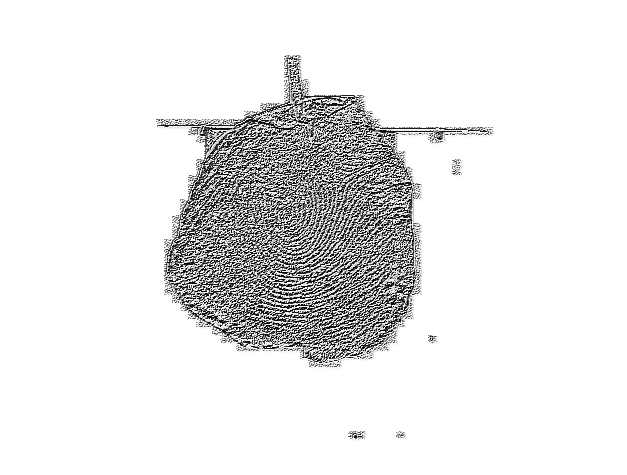
\includegraphics[width=100px]{images/fake53otsulbp.png}
    \caption{Fake fingerprint processed by LBP}
  \end{minipage}
  \hspace{0.3cm}
  \begin{minipage}[b]{0.3\linewidth}
    \centering
    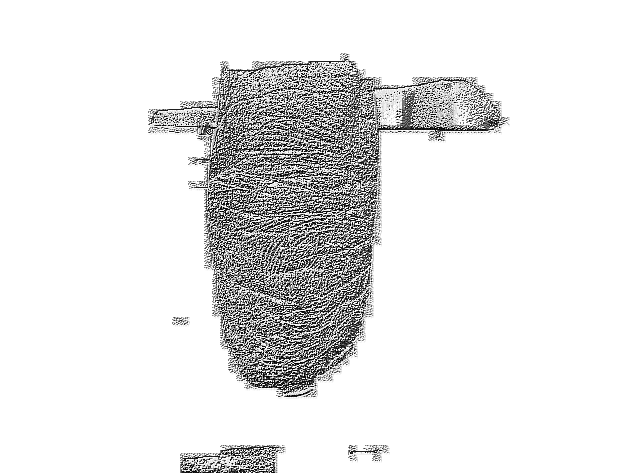
\includegraphics[width=100px]{images/Images29lbp.png}
    \caption{Live fingerprint processed by LBP}
  \end{minipage}
  \hspace{0.3cm}
    \begin{minipage}[b]{0.3\linewidth}
    \centering
    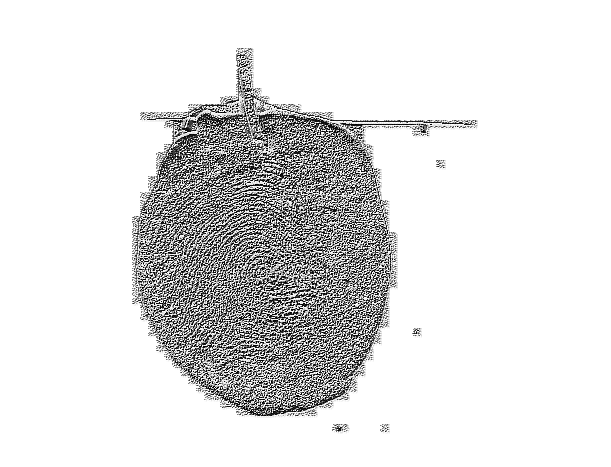
\includegraphics[width=100px]{images/fake44otsulbp.png}
    \caption{Fake fingerprint processed by LBP}
  \end{minipage}
\end{figure}

\subsection{Extracted vector based on Sobel and Laplacian operator}
Sobel and Laplacian methods work well as edge and texture detectors. Kernel $5x5$ was used for this feature extraction. We can extract Sobel only based on $x$ or $y$ axis. So we have two different results of horizontal and vertical Sobel operator. Then Laplacian image was extracted and characteristics were also added to this vector.

Vector contains features $f_1$ (contrast), $f_2$ (homogeneity), $f_3$ (energy), $f_4$ (correlation) of GLCM matrix for Sobel $x$ image $Sobelx$ , Sobel $y$ $Sobely$ image and Laplacian $Laplacian$ image.

This is the final extracted vector:

$$v = [f_1_{Sobelx}, f_2_{Sobelx}, f_3_{Sobelx}, f_4_{Sobelx}, f_1_{Sobely}, f_2_{Sobely}, f_3_{Sobely}, f_4_{Sobely}, f_1_{Laplacian}, f_2_{Laplacian}, f_3_{Laplacian}, f_4_{Laplacian}]$$

\begin{figure}[htbp]
  \begin{minipage}[b]{0.3\linewidth}
    \centering
    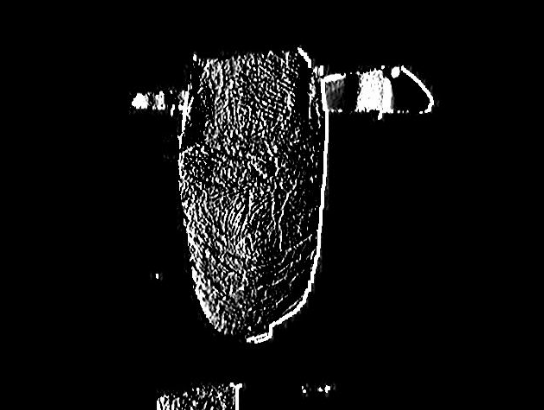
\includegraphics[width=100px]{images/sobelxlive.png}
    \caption{Sobel of x-axis of live fingerprint}
  \end{minipage}
  \hspace{0.3cm}
  \begin{minipage}[b]{0.3\linewidth}
    \centering
    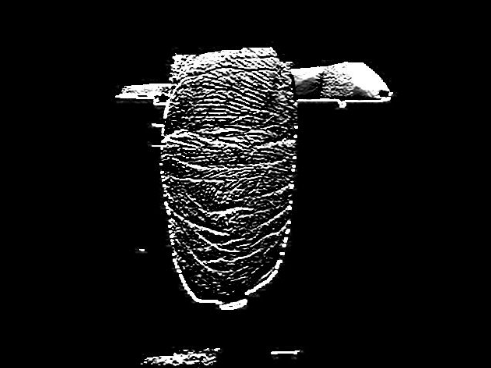
\includegraphics[width=100px]{images/sobelylive.png}
    \caption{Sobel of y-axis of live fingerprint}
  \end{minipage}
  \hspace{0.3cm}
    \begin{minipage}[b]{0.3\linewidth}
    \centering
    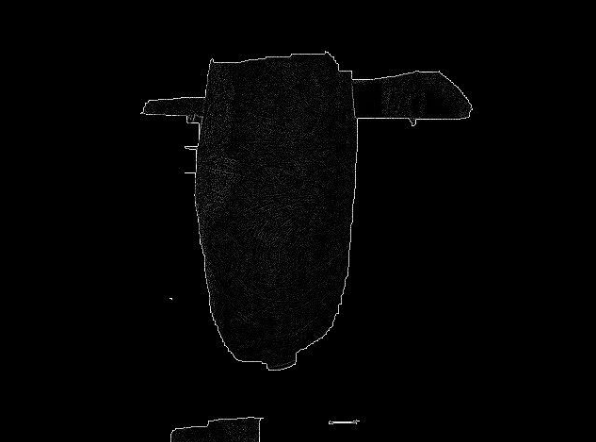
\includegraphics[width=100px]{images/laplacianlive.png}
    \caption{Laplacian of live fingerprint}
  \end{minipage}
\end{figure}

\begin{figure}[htbp]
  \begin{minipage}[b]{0.3\linewidth}
    \centering
    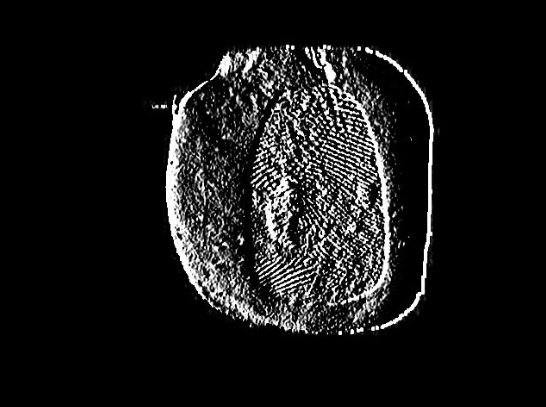
\includegraphics[width=100px]{images/sobelxfingerprint.png}
    \caption{Sobel of x-axis of fake fingerprint}
  \end{minipage}
  \hspace{0.3cm}
  \begin{minipage}[b]{0.3\linewidth}
    \centering
    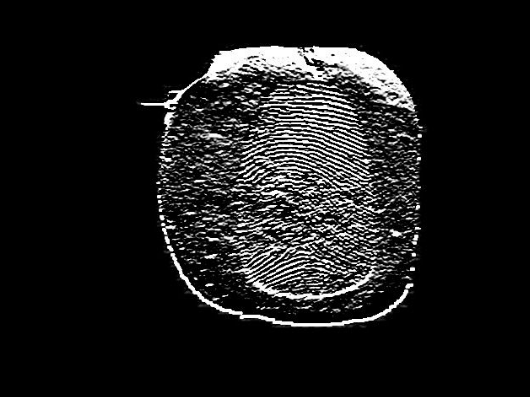
\includegraphics[width=100px]{images/sobelyfingerprint.png}
    \caption{Sobel of y-axis of fake fingerprint}
  \end{minipage}
  \hspace{0.3cm}
    \begin{minipage}[b]{0.3\linewidth}
    \centering
    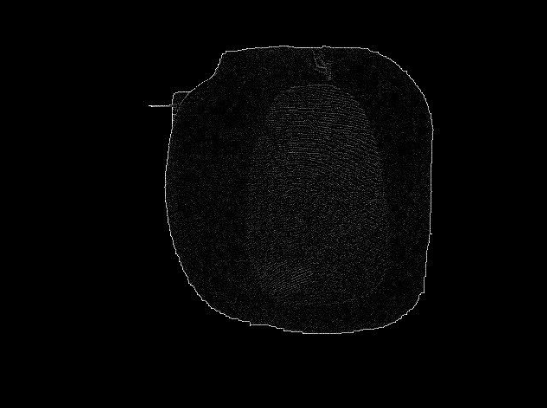
\includegraphics[width=100px]{images/laplacianfingerprint.png}
    \caption{Laplacian of fake fingerprint}
  \end{minipage}
\end{figure}

\subsection{Extracted vector based on Wavelet Transformation}
Wavelet processing with different wavelet families such as biorthogonal or Daubechies wavelets is also used in image processing. We have three details from image processed by wavelet transformation - horizontal $LH$, vertical $HL$ and diagonal $HH$. We can extract features from GLCM matrix for each detail. Features $f_1$, $f_2$, $f_3$, $f_4$ stands for same features from GLCM matrix as in previous vectors.

$$v = [f_1_{LH}, f_2_{LH}, f_3_{LH}, f_4_{LH}, f_1_{HL}, f_2_{HL}, f_3_{HL}, f_4_{HL}, f_1_{HH}, f_2_{HH}, f_3_{HH}, f_4_{HH}]$$

\begin{figure}[htbp]
    \centering
    \includegraphics[width=270px]{images/fake53bior15otsu.png}
    \caption{Wavelet transformation of fake image based on bior1.5 method }
\end{figure}

\section{Analyzing the images with same light }
During taking the dataset from touchless sensor, we use lights of different wavelength for taking the images. The lights were blue, green and red. The goal was to realize which light is most accurate for liveness detection. The all methods were also compared. Three methods for segmentation were used. First type of segmentation uses Otsu tresholding, which uses constant tresh based on particular image. The other two types of segmentation uses Gaussian and Mean adaptive tresholding, which is suitable for images with various light properties and the tresh isn't constant for whole image as with Otsu algorithm, but it changes for every pixel based on their neighbors.  

Below are some examples of images, how they were taken with our touchless fingerprint scanner.\\

\begin{figure}[htbp]
  \begin{minipage}[b]{0.3\linewidth}
    \centering
    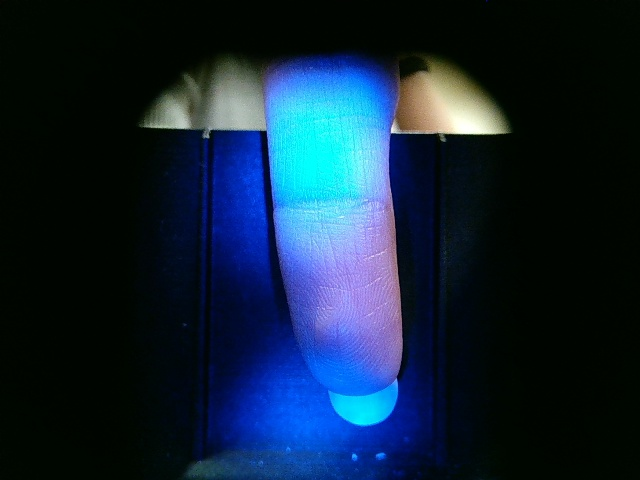
\includegraphics[width=100px]{images/live120.jpg}
    \caption{Image of live fingerprint with blue light}
  \end{minipage}
  \hspace{0.3cm}
  \begin{minipage}[b]{0.3\linewidth}
    \centering
    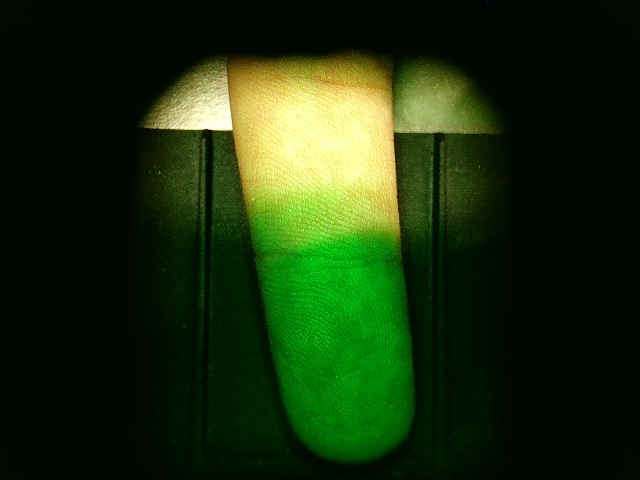
\includegraphics[width=100px]{images/live38.jpg}
    \caption{Image of live fingerprint with green light}
  \end{minipage}
  \hspace{0.3cm}
    \begin{minipage}[b]{0.3\linewidth}
    \centering
    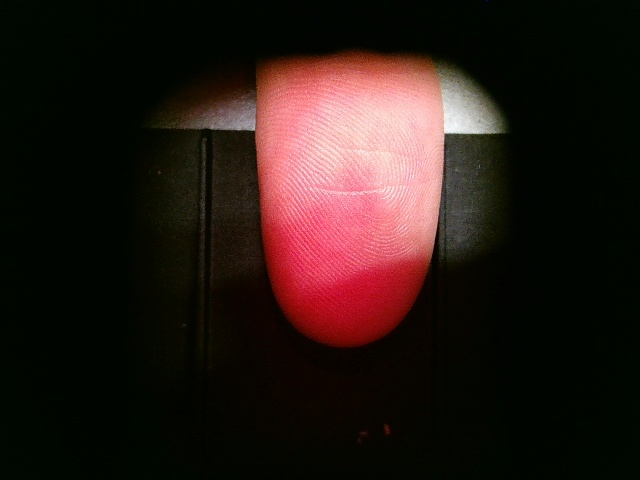
\includegraphics[width=100px]{images/live56.jpg}
    \caption{Image of live fingerprint with red light}
  \end{minipage}
\end{figure}

\begin{figure}[htbp]
  \begin{minipage}[b]{0.3\linewidth}
    \centering
    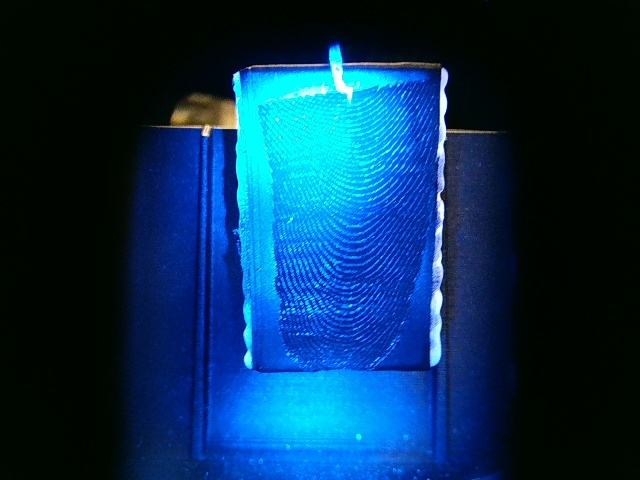
\includegraphics[width=100px]{images/fake23.jpg}
    \caption{Image of fake fingerprint with blue light}
  \end{minipage}
  \hspace{0.3cm}
  \begin{minipage}[b]{0.3\linewidth}
    \centering
    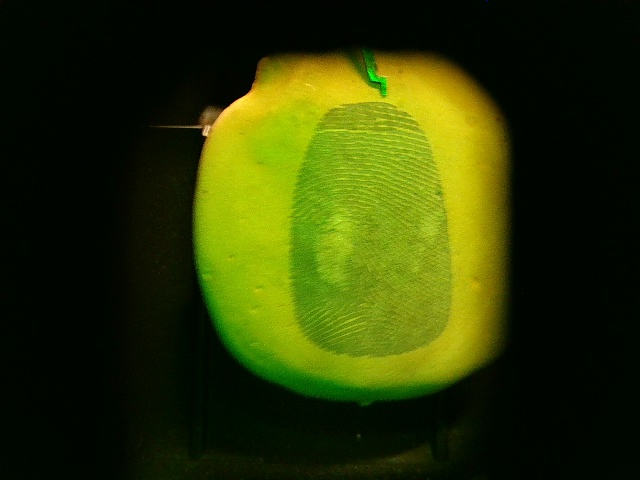
\includegraphics[width=100px]{images/fake64.jpg}
    \caption{Image of fake fingerprint with green light}
  \end{minipage}
  \hspace{0.3cm}
    \begin{minipage}[b]{0.3\linewidth}
    \centering
    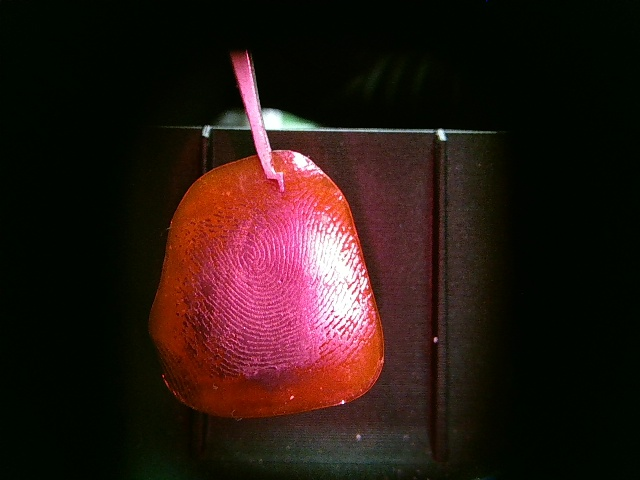
\includegraphics[width=100px]{images/fake47.jpg}
    \caption{Image of fake fingerprint with red light}
  \end{minipage}
\end{figure}

Each tested and trained dataset contains images with same light. These are datasets for blue, green and red images:
\begin{figure}[htbp]
    \centering
    \includegraphics[width=250px]{images/BlueLightImages.png}
    \caption{Dataset for images with blue light}
\end{figure}

\begin{figure}[htbp]
    \centering
    \includegraphics[width=250px]{images/GreenLightImages.png}
    \caption{Dataset for images with green light}
\end{figure}

\begin{figure}[htbp]
    \centering
    \includegraphics[width=250px]{images/RedLightImages.png}
    \caption{Dataset for images with red light}
\end{figure}

Each dataset was trained and tested with three different types of segmentation with different type of tresholding and Artificial Neural Network (ANN), Support Vector Machines (SVM) and Decision Trees were used for final classification, training and decision about results for dataset for testing.

\begin{figure}[!htbp]
    \centering
    \includegraphics[width=250px]{images/lightsClassifier.png}
    \caption{Table of average accuracy of various classifier }
\end{figure}

These are examples of various segmentation type based on three methods of threshold:\\
\begin{figure}[!htbp]
  \begin{minipage}[b]{0.3\linewidth}
    \centering
    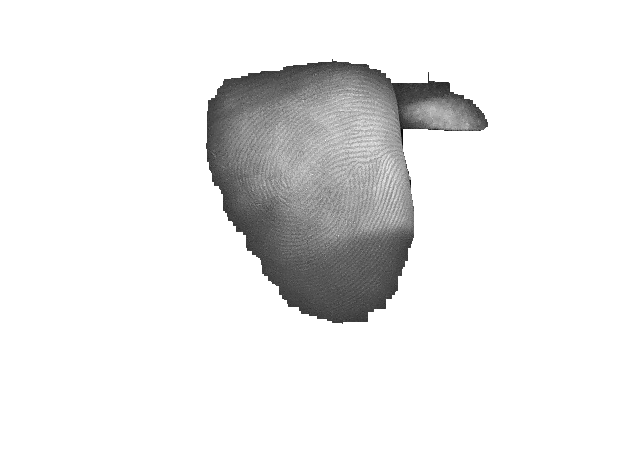
\includegraphics[width=100px]{images/Images14otsu.png}
    \caption{Segmentation with Otsu tresholding}
  \end{minipage}
  \hspace{0.3cm}
  \begin{minipage}[b]{0.3\linewidth}
    \centering
    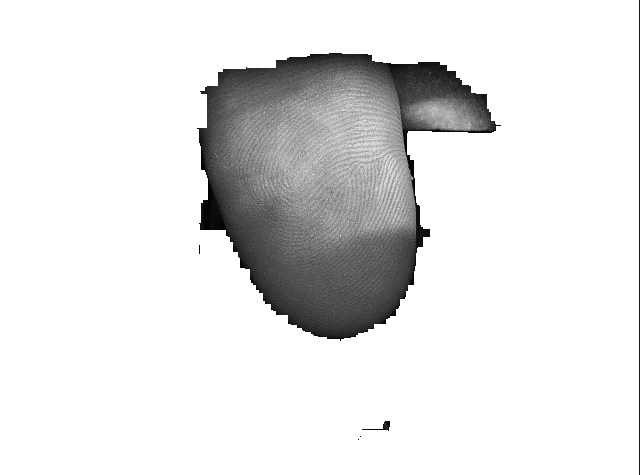
\includegraphics[width=100px]{images/Images14gauss.png}
    \caption{Segmentation with adaptive Gaussian tresholding}
  \end{minipage}
  \hspace{0.3cm}
    \begin{minipage}[b]{0.3\linewidth}
    \centering
    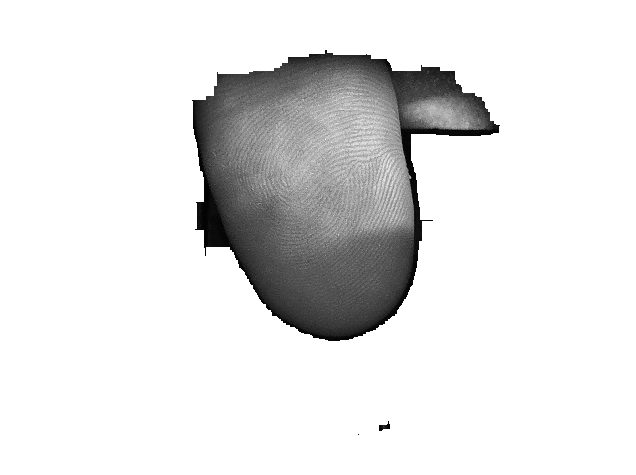
\includegraphics[width=100px]{images/Images14mean.png}
    \caption{Segmentation with adaptive Mean tresholding}
  \end{minipage}
\end{figure}

This is the rating of different segmentation based on their accuracy:
\begin{figure}[!htbp]
    \centering
    \includegraphics[width=200px]{images/lightsSegmentation.png}
    \caption{Table of average accuracy of various segmentation type}
\end{figure}
\\\\\\\\
Different wavelet families were used for Wavelet transformation. I used two wavelet transformation based on Daubechies wavelet family ($db2$, $db4$), three wavelets based on biorthogonal wavelet family ($bior1.3$, $bior2.4$, $bior1.5$) and one wavelet type based on reverse biorthogonal wavelet family ($rbio3.1$). We can compare not only different methods but also different types of wavelet transformation.

These are average accuracy of various used methods. For every method except Sobel method were used all three different types of segmentation, Sobel uses only Otsu tresholding because of better accuracy and ANN error function based on epochs. So we can compare all methods except Sobel with all segmentation types and then all methods including Sobel with only Otsu segmentation.

\begin{figure}[!htbp]
    \centering
    \includegraphics[width=200px]{images/allSegmentationLightsMethods.png}
    \caption{Average accuracy for methods with use of all segmentation techniques}
\end{figure}

\begin{figure}[!htbp]
    \centering
    \includegraphics[width=200px]{images/AllLightsOnlyOtsu.png}
    \caption{Average accuracy for all methods with use of segmentation with Otsu thresholding}
\end{figure}

We can see that for separate datasets with different lights is most suitable use a vector based on LBP. Method based on Sobel and Laplacian method is also quite accurate and also faster than processing LBP algorithm. The advantage of wavelet transformation is wide list of various wavelet families (biorthogonal, reverse biorthogonal, Daubechies, Symlets, Coiflets) but the processing the image with wavelet and get horizontal, vertical and diagonal detail is slower especially with large datasets.

Finally we can find out which color gives the best accuracy and is the most reliable for liveness detection on touchless device.

\begin{figure}[!htbp]
    \centering
    \includegraphics[width=200px]{images/accuracyLights.png}
    \caption{Average accuracy for all tested datasets with blue, green and red lights}
\end{figure}

We can see that the best accuracy have the images with red light. Therefore they are most suitable for liveness detection on our device. It is commonly known that green light reflects the biggest light amount back, so it is most suitable for measure reflected light with some specialized device, but when it comes to software texture analysis, the red light can shine through finger with least reflected light back, so the texture of fingerprint is most accurate without minimal reflections.

\section{Analyzing images with mix of images with all lights}
The all datasets from previous chapter are combined into one dataset, so we have dataset with mix of images with all the different lights.

Similar to analyzing data set with various lights, we want to figure out what type of segmentation, classifier and method is most suitable for liveness detection, when we have large dataset with different lights.

\end{document}
